\documentclass[11pt,aspectratio=169,handout]{beamer}

\usetheme{Singapore}
\usecolortheme{orchid}

\usepackage[utf8]{inputenc}
\usepackage[russian]{babel}
\usepackage{amsmath}
\usepackage{amsfonts}
\usepackage{amssymb}
\usepackage{graphicx}
\usepackage{bibentry}
\usepackage{wasysym}
\usepackage[most]{tcolorbox}
\usepackage[normalem]{ulem}

\usepackage{hyperref}

\definecolor{info}{RGB}{62, 180, 137}
\definecolor{warn}{RGB}{128, 0, 0}

\author{Николай Анохин}
\title{Нерешенные проблемы и новые направления}

\logo{
\includegraphics[width=.05\textwidth]{images/ok_logo.png}}

\AtBeginSection[]{
  \begin{frame}
  \vfill
  \centering
  \begin{beamercolorbox}[sep=8pt,center,shadow=true,rounded=true]{title}
    \usebeamerfont{title}\insertsectionhead\par
  \end{beamercolorbox}
  \vfill
  \end{frame}
}

\begin{document}

{
\setbeamertemplate{headline}{}

\begin{frame}
\titlepage
\end{frame}

%\begin{frame}
%\tableofcontents
%\end{frame}

}

\begin{frame}{Контекст}

\begin{center}
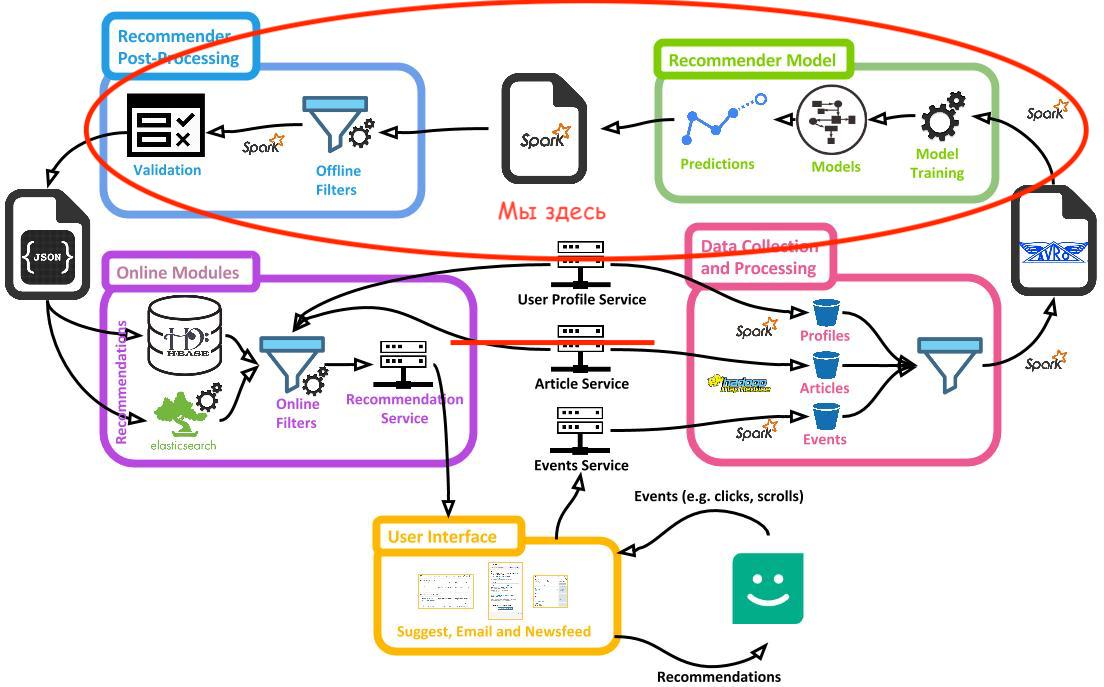
\includegraphics[scale=0.23]{images/mendeley.jpeg}
\end{center}

\end{frame}

\begin{frame}{Что мы уже умеем}

\begin{columns}
\begin{column}{0.55\textwidth}
\begin{center}
\begin{tcolorbox}[colback=info!5,colframe=info!80,title=]
\begin{large}
\[
\hat r_{ui} = f_{\theta}(x_u, x_i, x_c)
\]
\end{large}
\end{tcolorbox}\end{center}
\end{column}

\begin{column}{0.35\textwidth} 
\begin{center}

\includegraphics[scale=0.4]{images/simple.jpeg}
\end{center}
\end{column}
\end{columns}

\vfill

Проблемы
\begin{enumerate}[<+->]
\item Оцениваем айтемы по-отдельности, а показываем по несколько (лентой)
\item Модель не объясняет, почему именно эти айтемы подходят пользователю
\item Смещение между распределениями на обучении и применении
\item {\color{blue} Не учитывается долгострочный эффект рекомендаций}
\end{enumerate}

\end{frame}

\section{Разнообразие в рекомендательных системах}

\begin{frame}{Разнообразие / Diversity}

\begin{center}
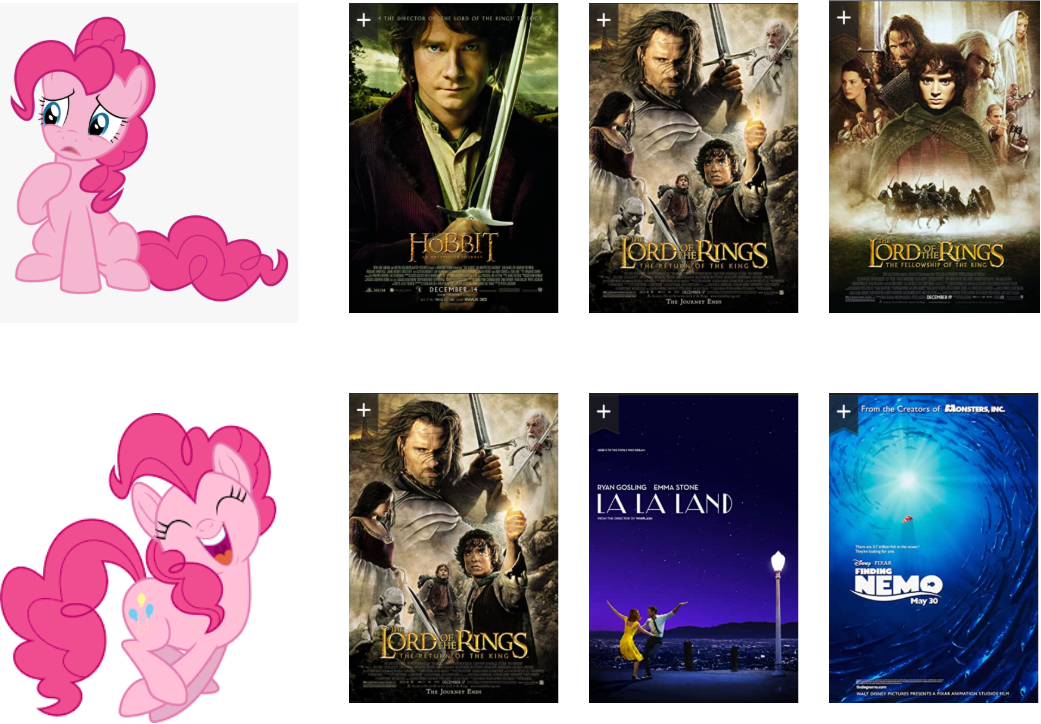
\includegraphics[scale=0.22]{images/diversity.png}
\end{center}

\end{frame}

\begin{frame}{Набираем айтемы с разными аспектами}

$f$ - аспект (признак) айтема, $p(f | i)$ -- вероятность найти аспект у айтема $i$

\vfill

Распределение аспекта у пользователя

\[
p(f | u) = \frac{\sum_{i \in I_u} p(f | i)}{|I_u|}  
\]

Распределение аспекта в рекомендациях
\[
q(f | u) = \frac{\sum_{i \in RL} p(f | i)}{|RL|}
\]

\begin{tcolorbox}[colback=info!5,colframe=info!80,title=]
Формируем список так, чтобы $q(f | u)$ совпало с $p(f | u)$
\end{tcolorbox}

\end{frame}

\begin{frame}{Жадное переранжирование}

\begin{tcolorbox}[colback=info!5,colframe=info!80,title=]
Добавляем в список рекомендаций айтем с максимальным значением
\[
(1 - \lambda) \cdot s(u, i) + \lambda \cdot gain(i, RL),
\]
пока не получим список нужной длины.
\end{tcolorbox}

\vfill

\begin{itemize}
\item $s(u, i)$ -- релевантность айтема $i$ для пользователя $u$ 
\item $gain(i, RL) = div(RL \cup \{i\}) - div(RL)$ -- улучшение разнообразия при добавлении айтема
\item $\lambda$ -- гиперпараметр
\end{itemize}

\end{frame}

\begin{frame}{A Comparison of Calibrated and Intent-Aware Recommendations \cite{BRIDGE}}
\begin{center}
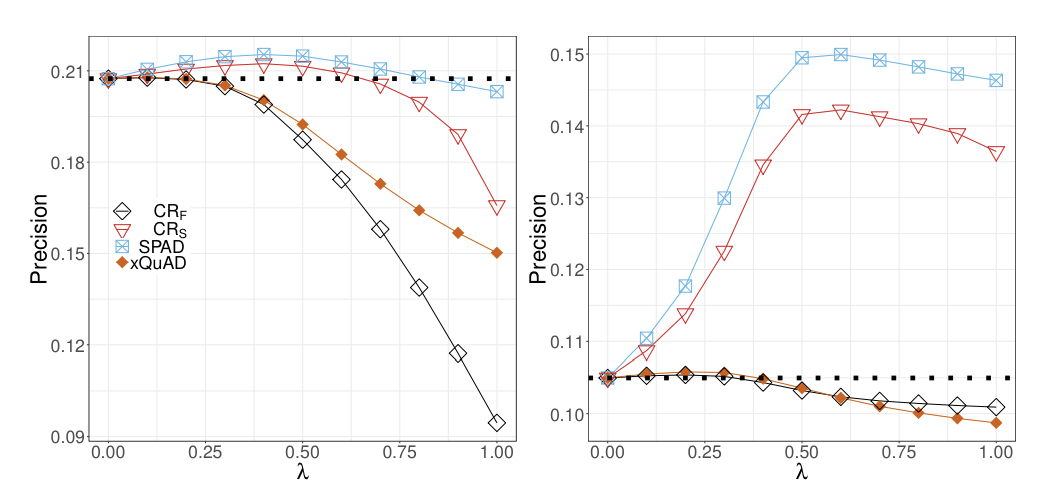
\includegraphics[scale=0.5]{images/spad.png}
\end{center}
\end{frame}

\begin{frame}{Учим разнообразие вместе с моделью 1}

\begin{center}
Controllable Multi-Interest Framework for Recommendation \cite{ALIBABA}
\end{center}

\begin{columns}
\begin{column}{0.45\textwidth}
\begin{center}
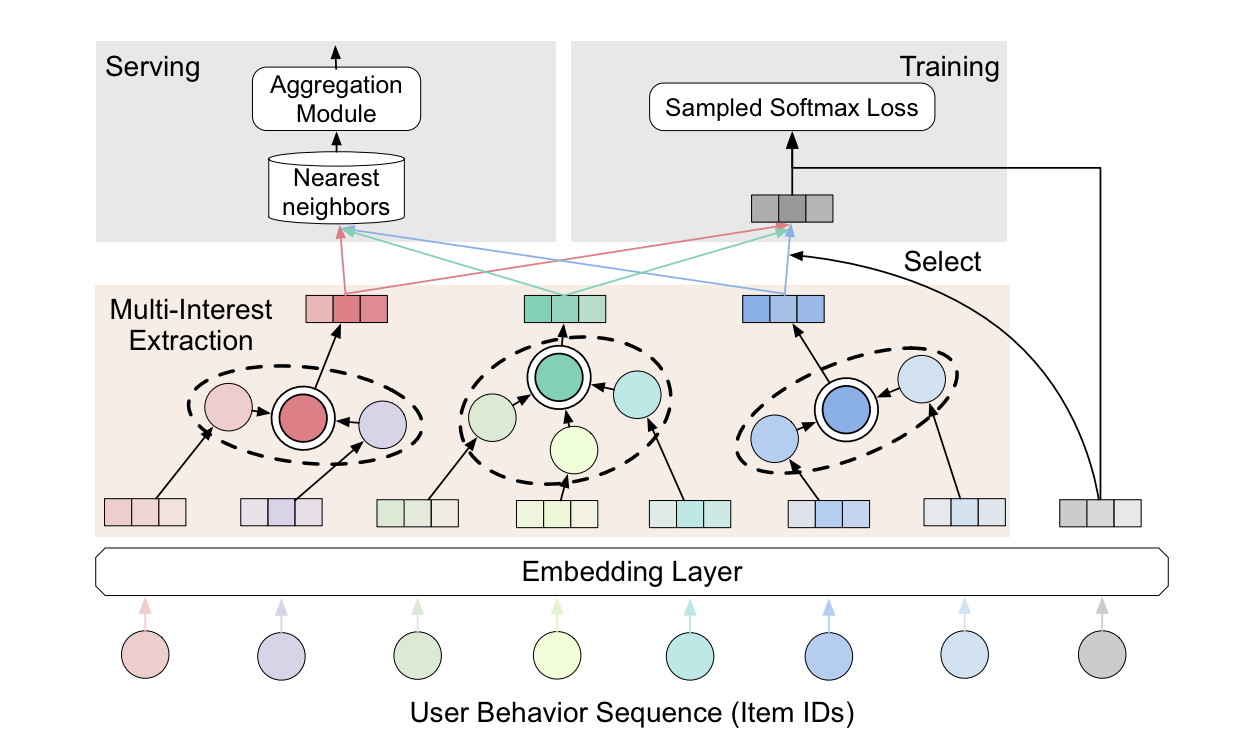
\includegraphics[scale=0.3]{images/alibaba.png}
\end{center}
\end{column}

\begin{column}{0.45\textwidth} 
\begin{center}
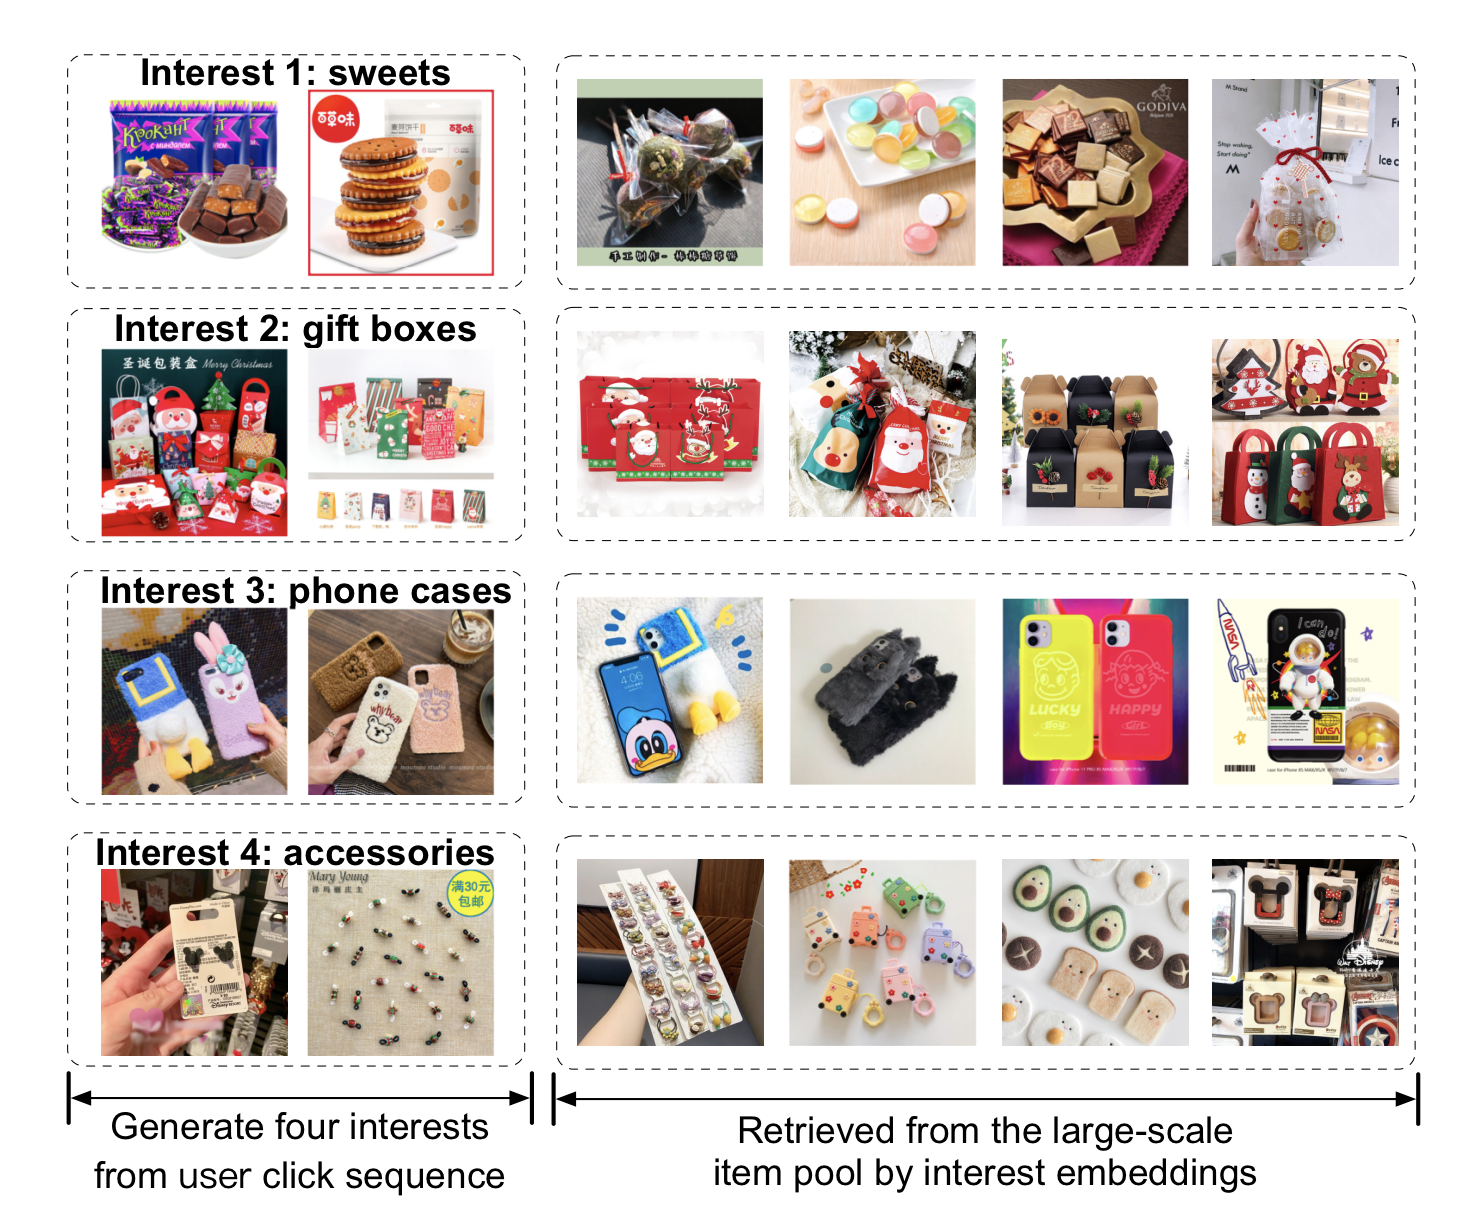
\includegraphics[scale=0.2]{images/divres.png}
\end{center}
\end{column}
\end{columns}

\end{frame}

\begin{frame}{Учим разнообразие вместе с моделью 2}

\begin{center}
Managing Diversity in Airbnb Search \cite{AIRBNB}
\end{center}

\begin{columns}

\begin{column}{0.45\textwidth}
\begin{center}
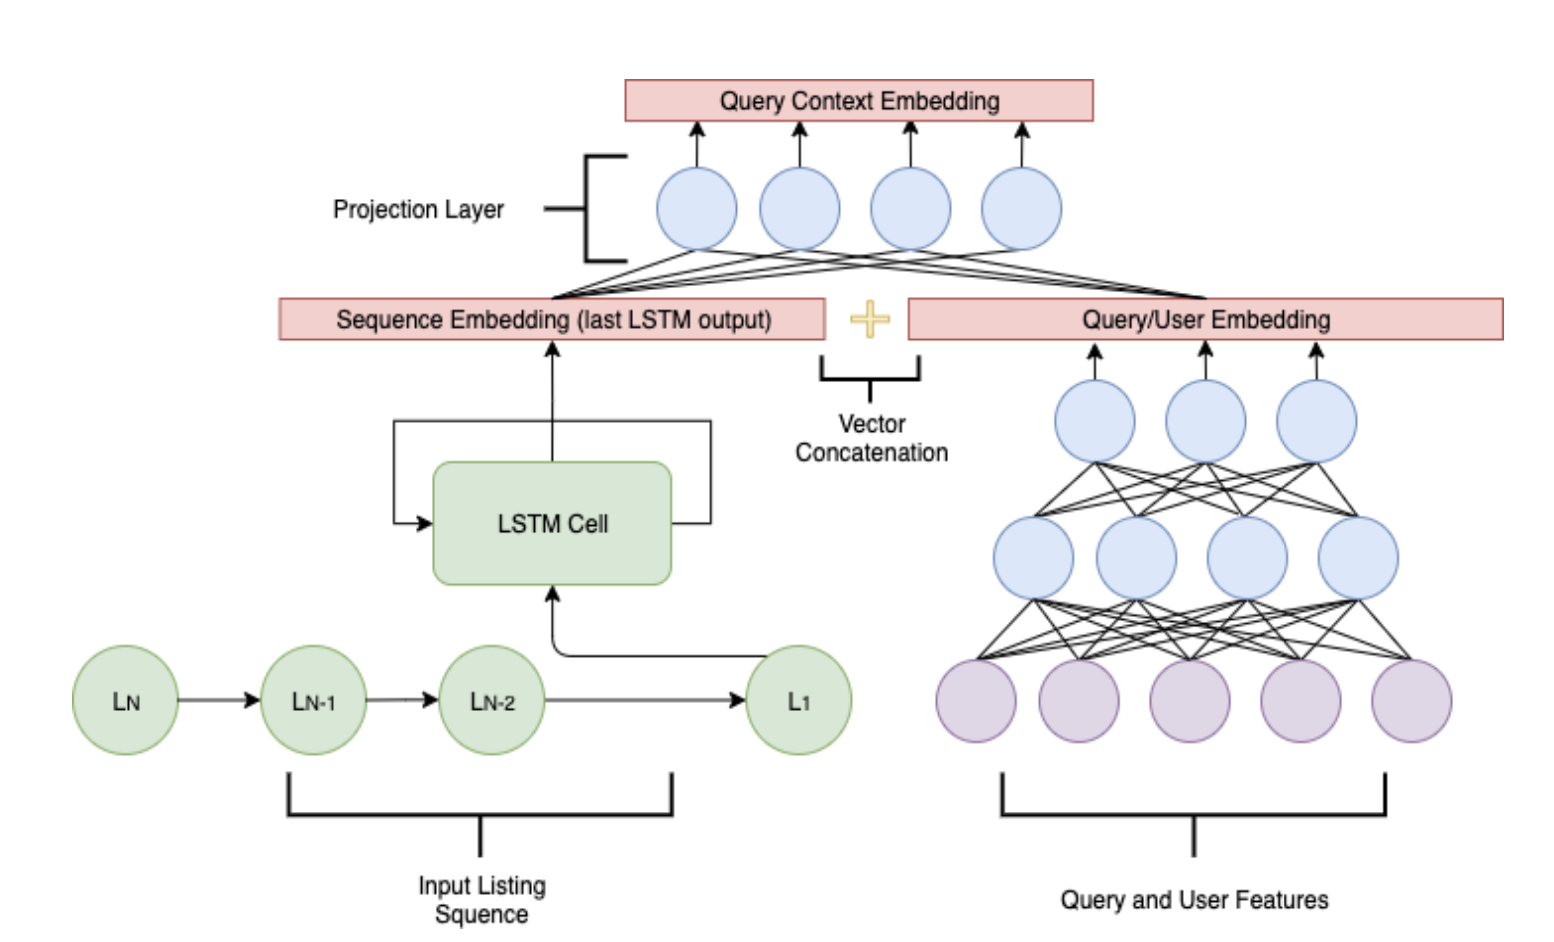
\includegraphics[scale=0.25]{images/airbnb2.png}
\end{center}
\end{column}

\begin{column}{0.45\textwidth} 
\begin{center}
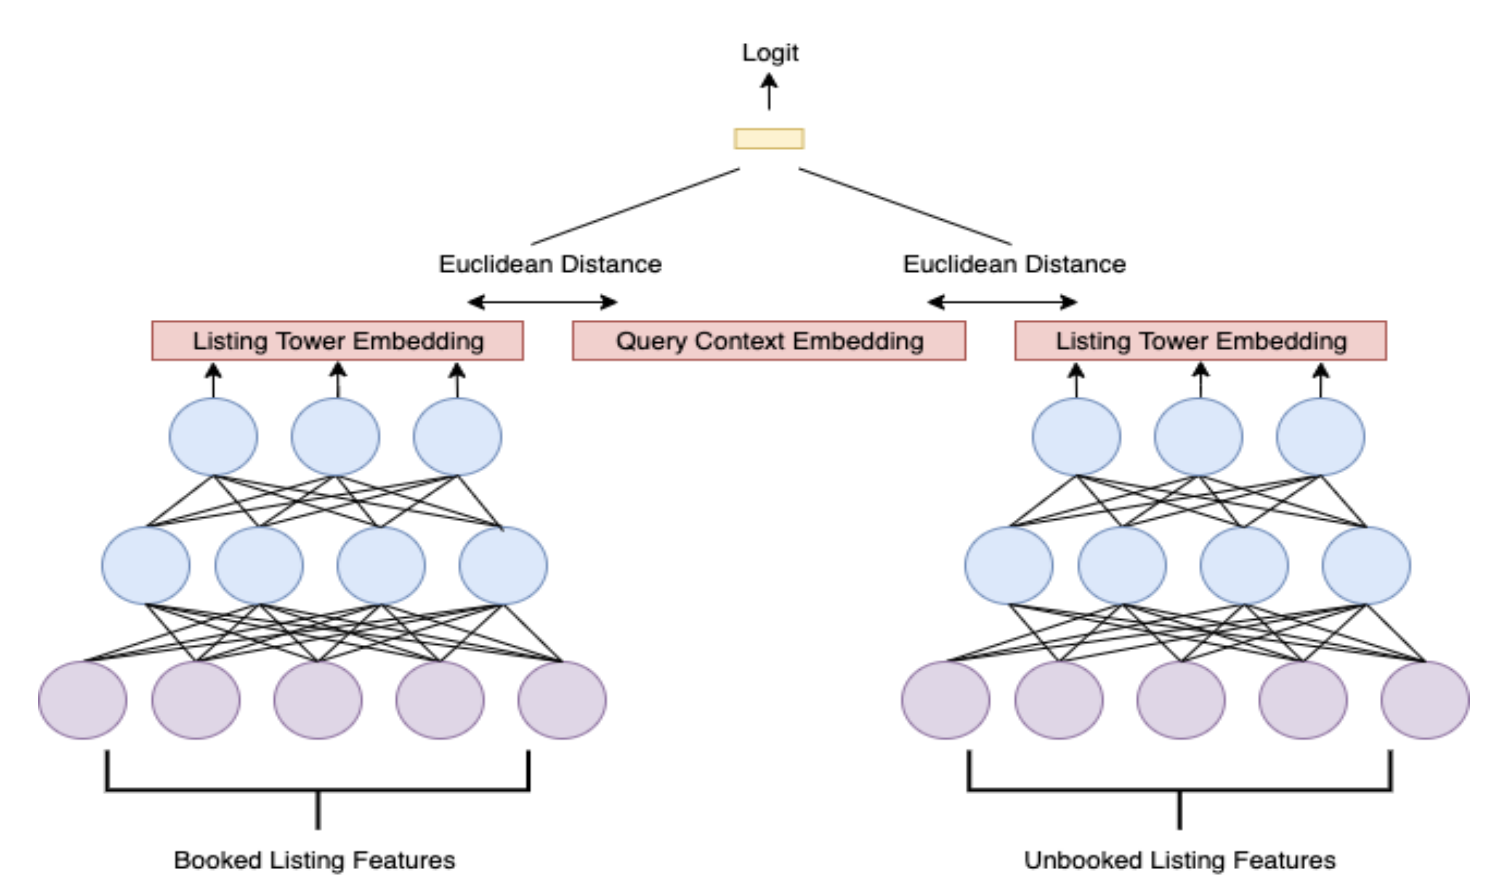
\includegraphics[scale=0.25]{images/airbnb.png}
\end{center}
\end{column}

\end{columns}

\end{frame}

\begin{frame}{}

\begin{tcolorbox}[colback=info!5,colframe=info!80,title=]
Из-за поточечного предсказания релевантности, приходится дополнительно разнообразить списки рекомендаций
\end{tcolorbox}

\begin{tcolorbox}[colback=info!5,colframe=info!80,title=]
Необходимость разнообразия обосновывается A/B экспериментом
\end{tcolorbox}

\end{frame}

\section{Объяснение рекомендаций}

\begin{frame}{Объяснения}

\begin{center}
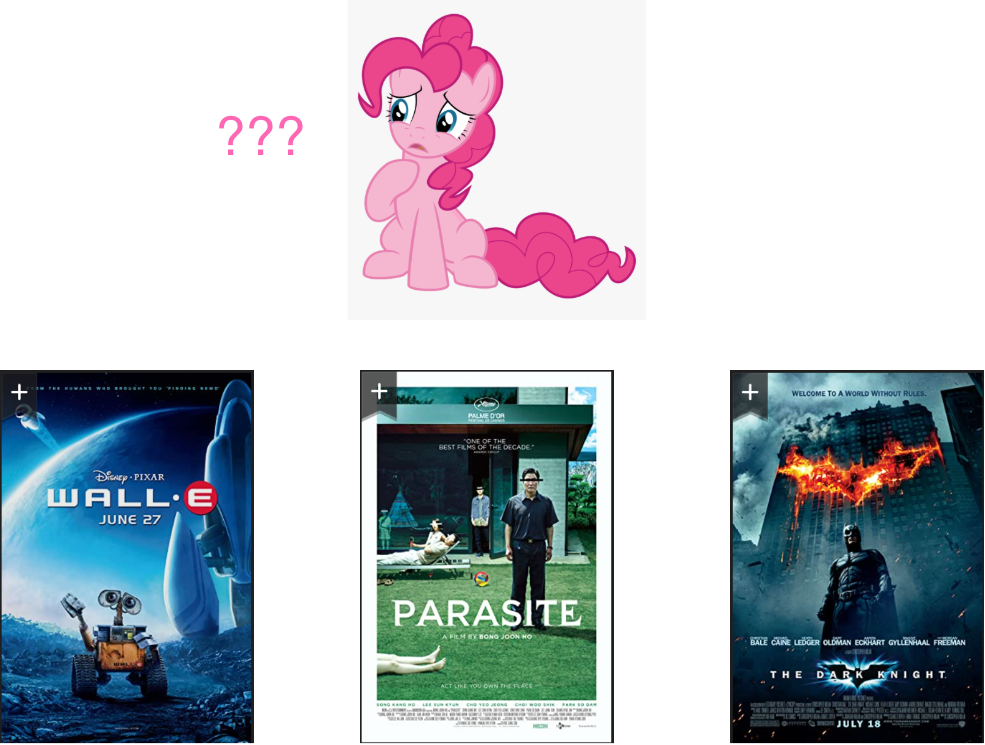
\includegraphics[scale=0.22]{images/explainability-1.png}
\end{center}

\end{frame}

\begin{frame}{Объяснения}

\begin{center}
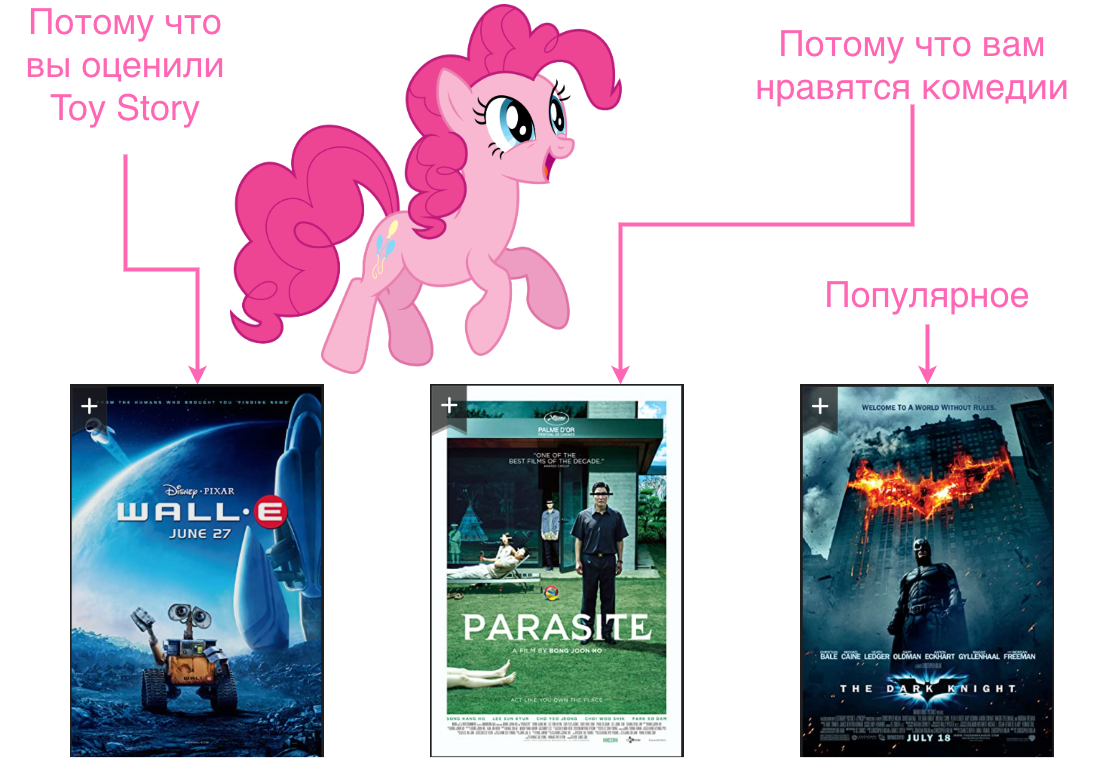
\includegraphics[scale=0.22]{images/explainability-2.png}
\end{center}

\end{frame}

\begin{frame}{Зачем объяснять рекомендации?}

\begin{enumerate}[<+->]
\item Прозрачность: объяснить пользователю, как работает система
\item Контролируемость: позволить пользователю исправить ошибки
\item Доверие: убедить пользователя, что система работает правильно
\item Убеждение: мотивировать пользователя к покупке
\item Полезность: помочь пользователю принять правильное решение
\item Эффективность: помочь пользователю принять решение быстро
\end{enumerate}

\end{frame}

\begin{frame}

\begin{tcolorbox}[colback=info!5,colframe=info!80,title=Case-based]
Because you have selected or highly rated: Movie A
\end{tcolorbox}

\vfill

\begin{center}
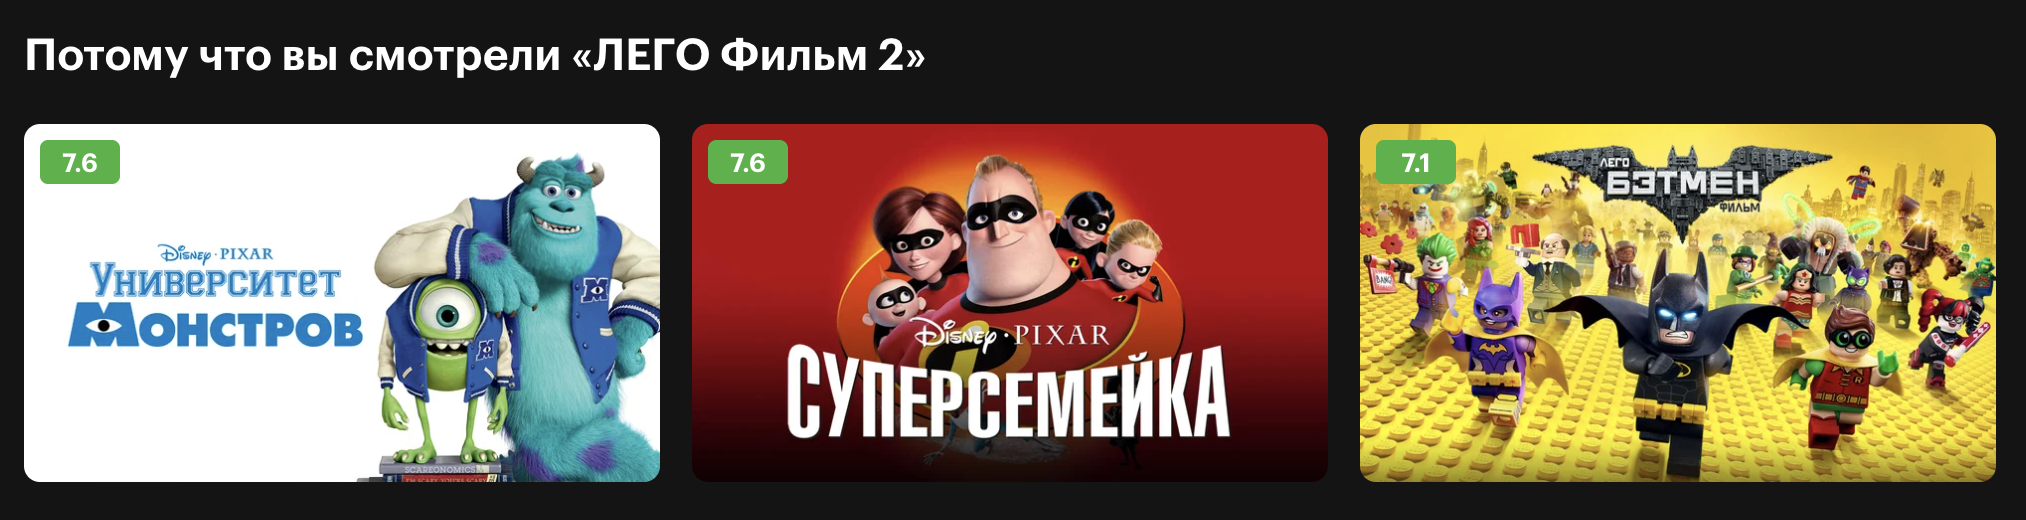
\includegraphics[scale=0.3]{images/netflix.png}
\end{center}

\end{frame}

\begin{frame}

\begin{tcolorbox}[colback=info!5,colframe=info!80,title=Collaborative]
Customers Who Bought This Item Also Bought A
\end{tcolorbox}

\vfill

\begin{center}
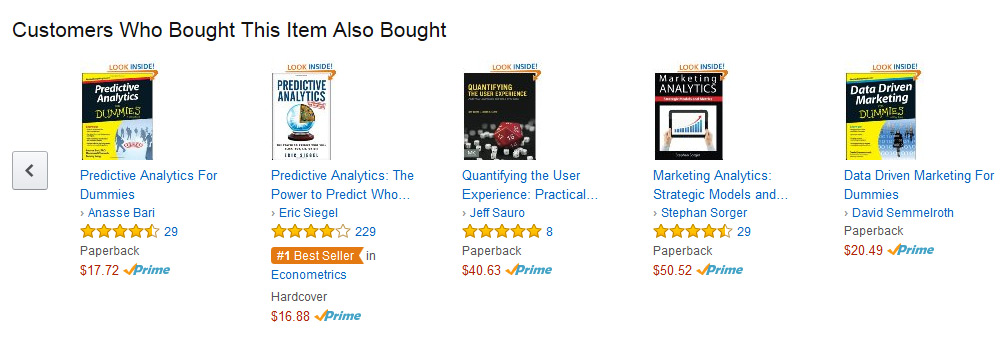
\includegraphics[scale=0.3]{images/amazon.jpeg}
\end{center}

\end{frame}

\begin{frame}

\begin{tcolorbox}[colback=info!5,colframe=info!80,title=Content-based]
Recommended because you said liked science fiction
\end{tcolorbox}

\vfill

\begin{center}

\includegraphics[scale=0.3]{images/facebook.png}
\end{center}

\end{frame}

\begin{frame}

\begin{tcolorbox}[colback=info!5,colframe=info!80,title=Knowledge-based]
Less Memory and Lower Resolution and Cheaper
\end{tcolorbox}

\vfill

\begin{center}
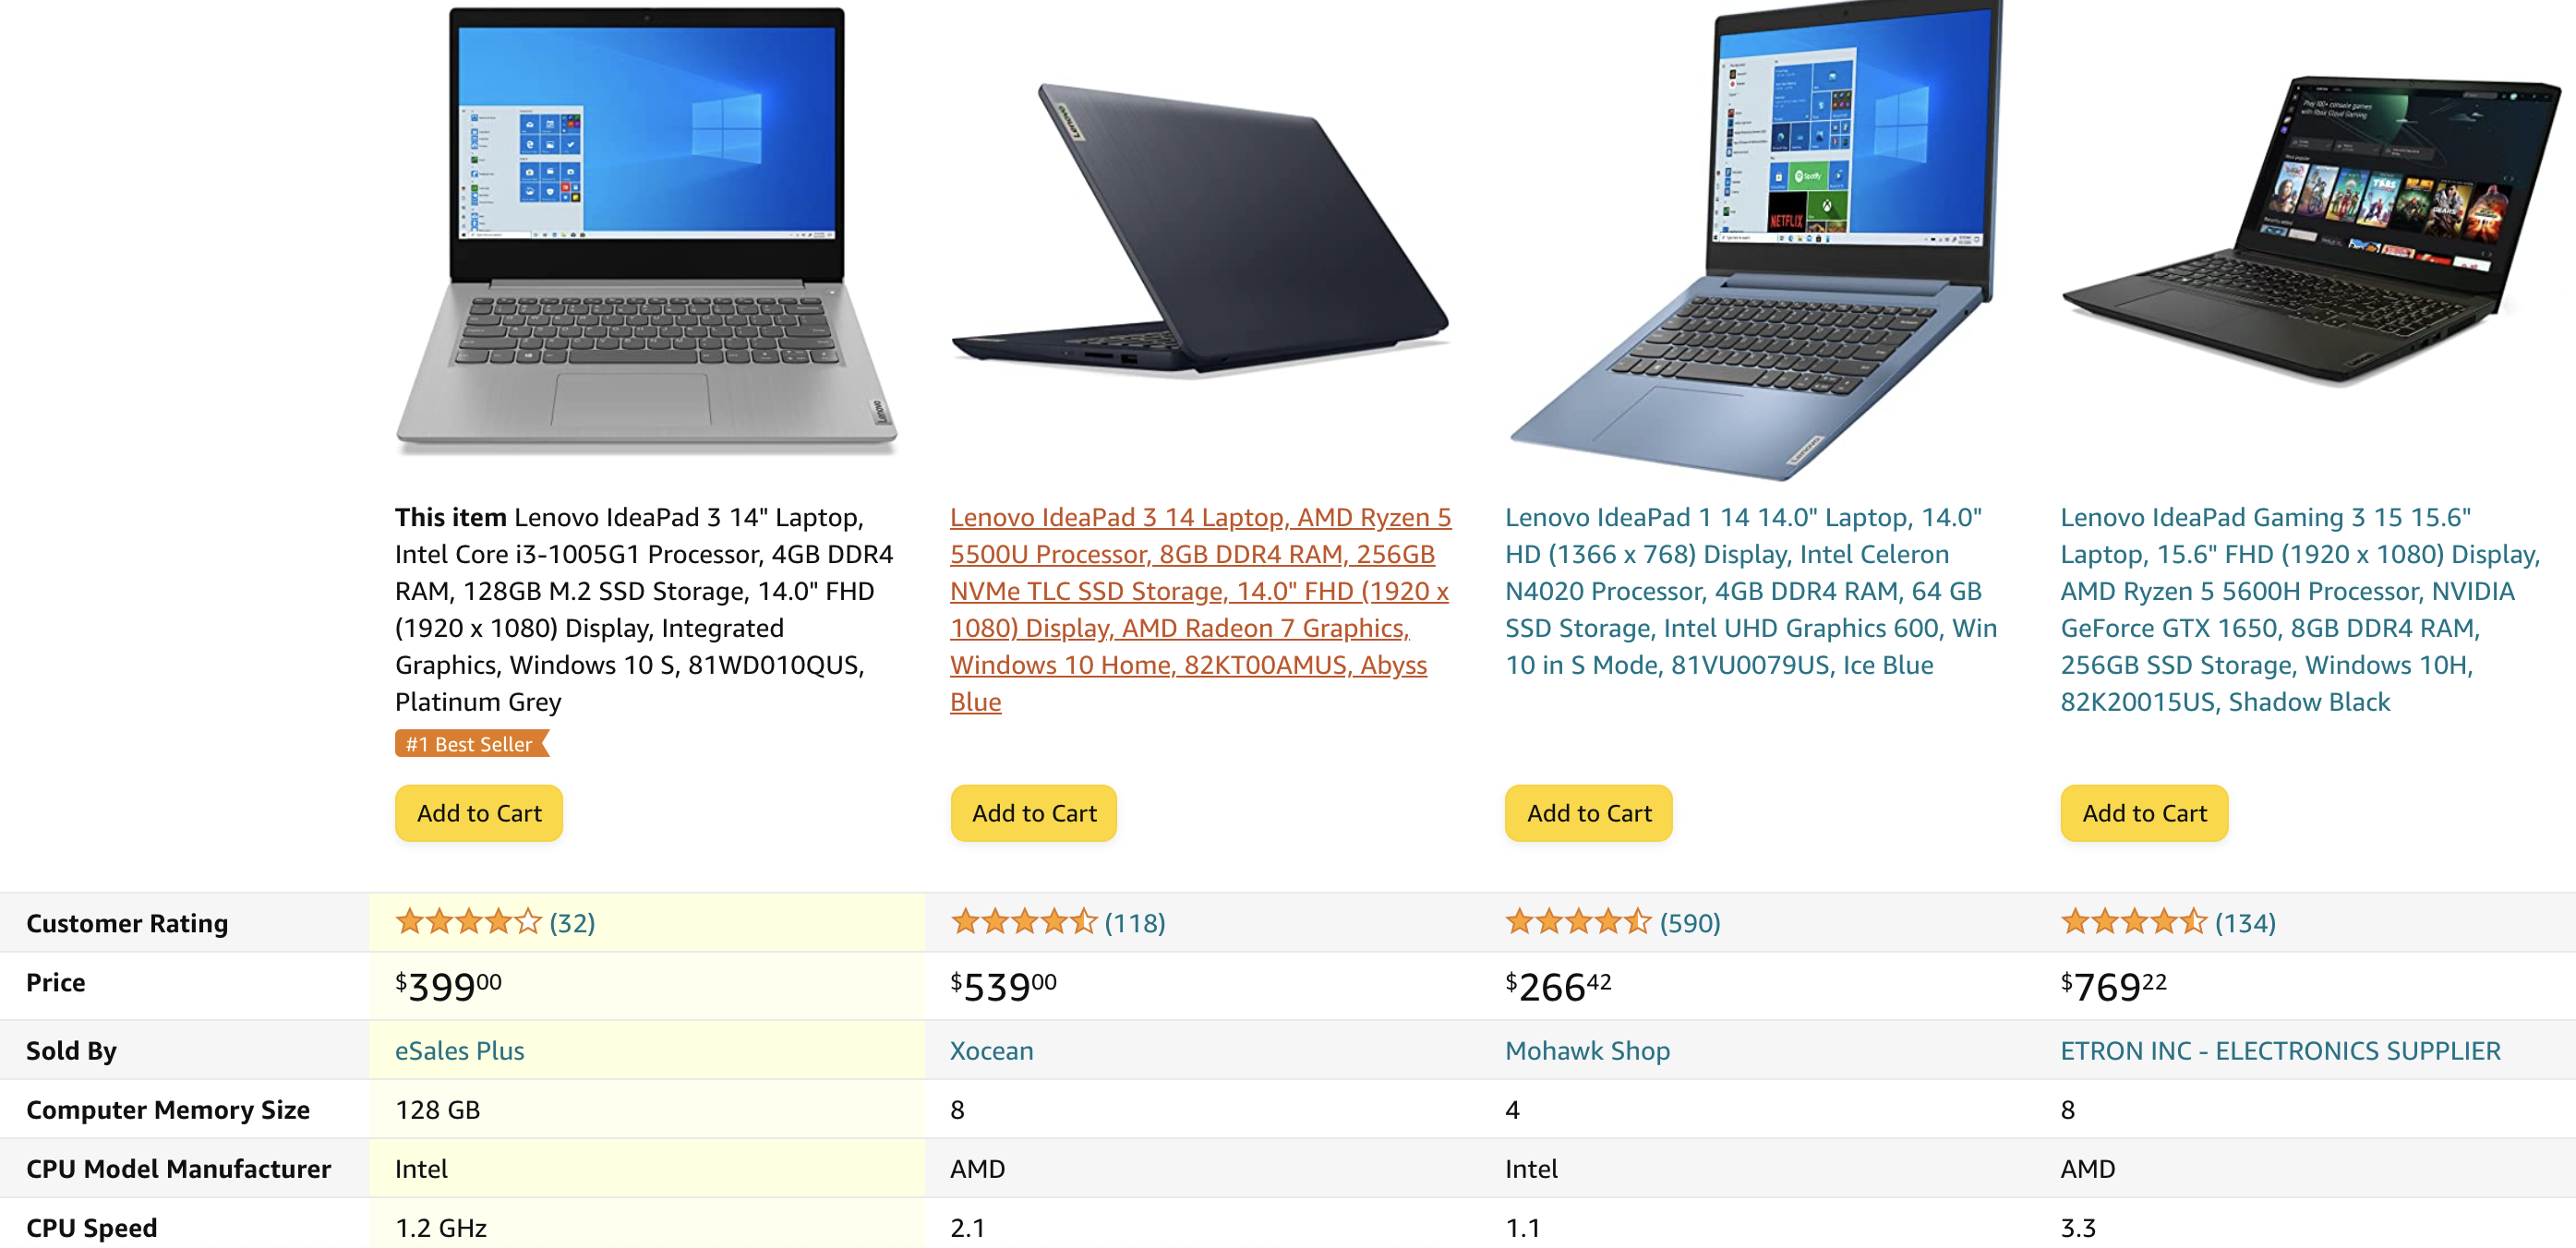
\includegraphics[scale=0.2]{images/amazon2.png}
\end{center}

\end{frame}

\begin{frame}{Explore, Exploit, and Explain: \\ Personalizing Explainable Recommendations with Bandits \cite{EX3}}

\begin{columns}
\begin{column}{0.4\textwidth}
\begin{center}
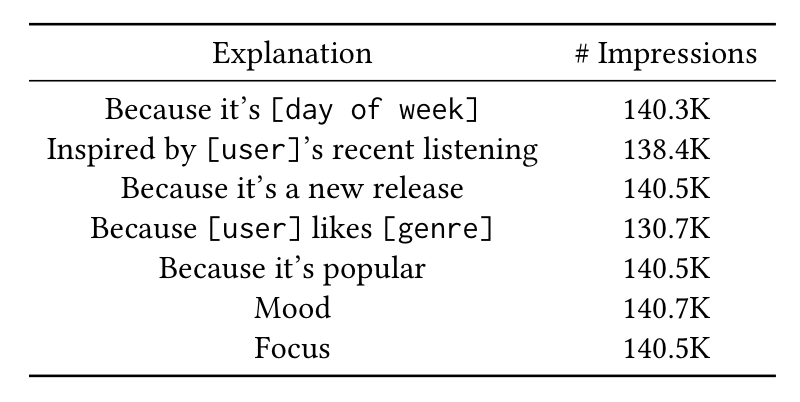
\includegraphics[scale=0.4]{images/spotify.png}
\end{center}
\end{column}

\begin{column}{0.5\textwidth}
\[
r(j, e, x) = \sigma(\theta_{global} + \theta_{j} \times 1_j + \theta_e \times 1_e + \theta_x \times 1_x)
\]
\end{column}
\end{columns}

\end{frame}

\begin{frame}{Why I like it: Multi-task Learning for Recommendation and Explanation \cite{GAN}}

\begin{center}
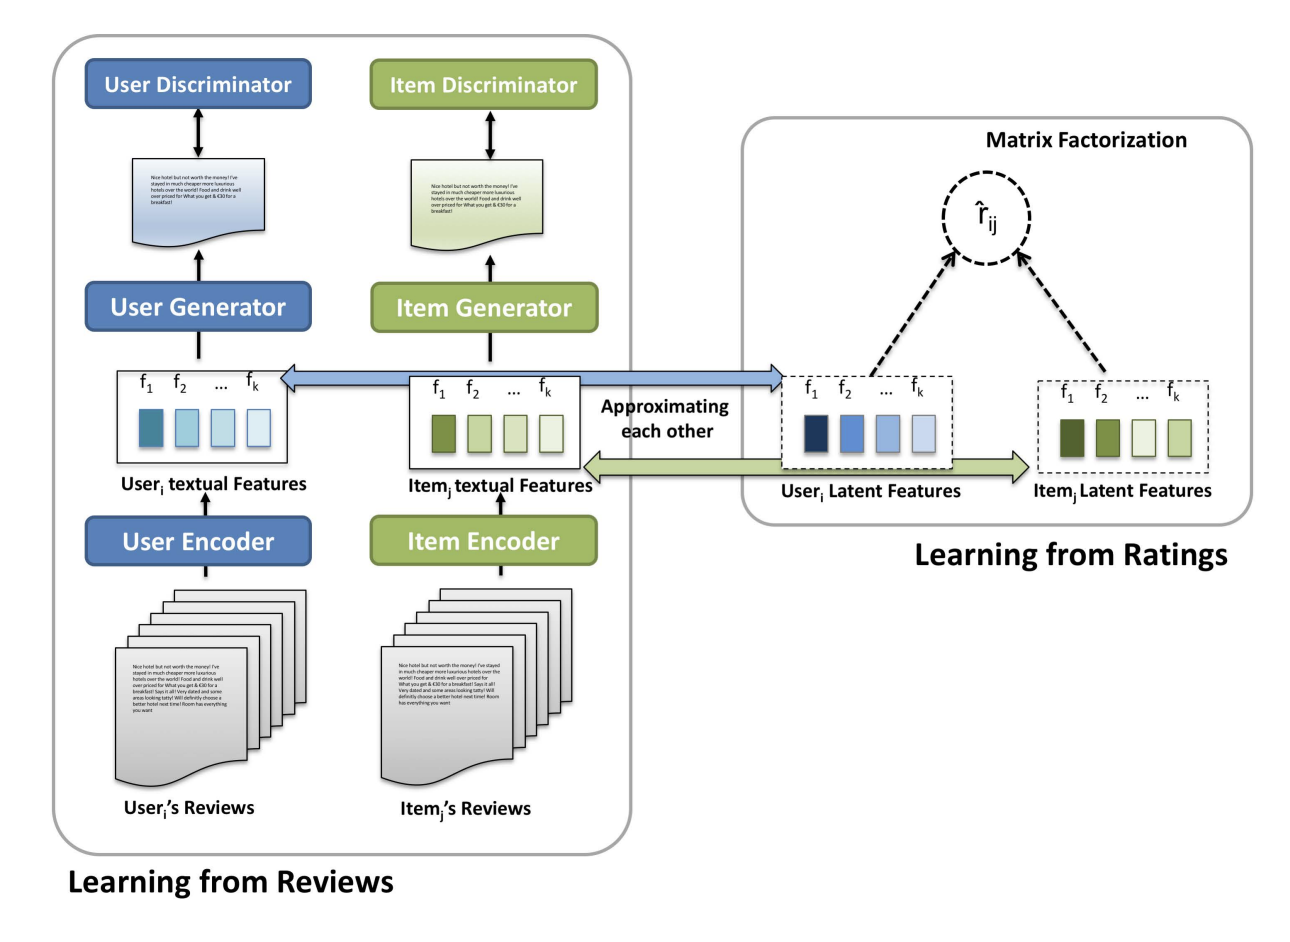
\includegraphics[scale=0.4]{images/gan.png}
\end{center}

\end{frame}

\begin{frame}

\begin{tcolorbox}[colback=info!5,colframe=info!80,title=]
Если хотим делать объяснения рекомендаций, нужно ответить на вопросы:
\begin{itemize}
\item Какую цель мы достигнем объяснениями?
\item Какие объяснения можно получить из модели?
\item Как правильно представить объяснения пользователю?
\end{itemize}
\end{tcolorbox}

\end{frame}

\section{Смещения}

\begin{frame}{Удачные рекомендации}

\begin{center}
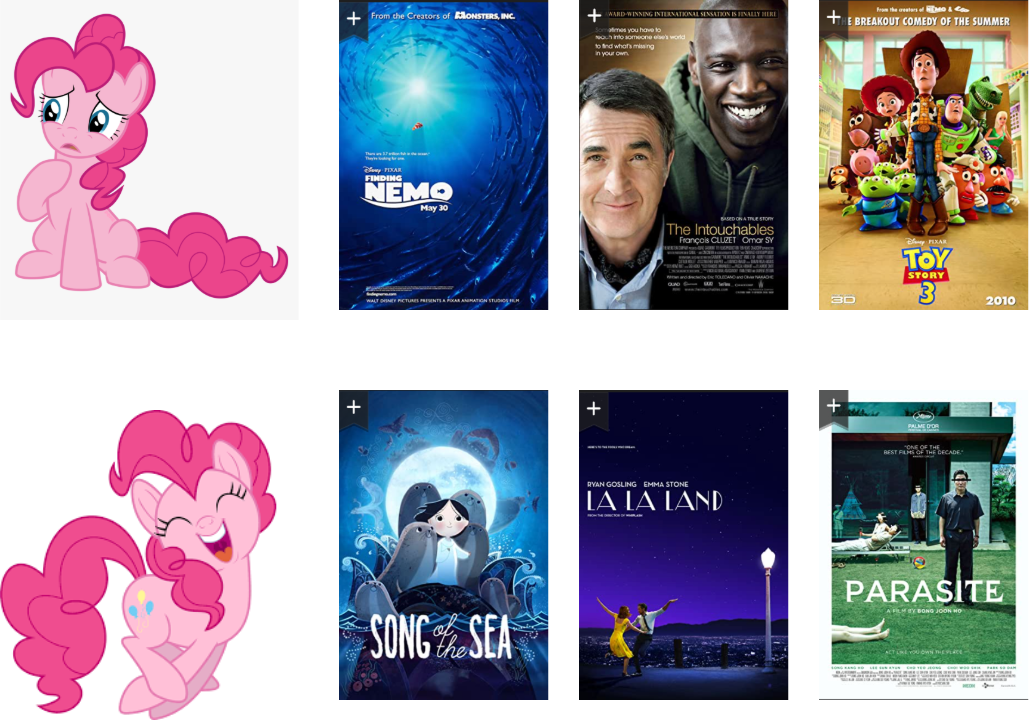
\includegraphics[scale=0.22]{images/serendipity-pony.png}
\end{center}

\end{frame}

\begin{frame}{Пример self-selection bias}

\begin{center}
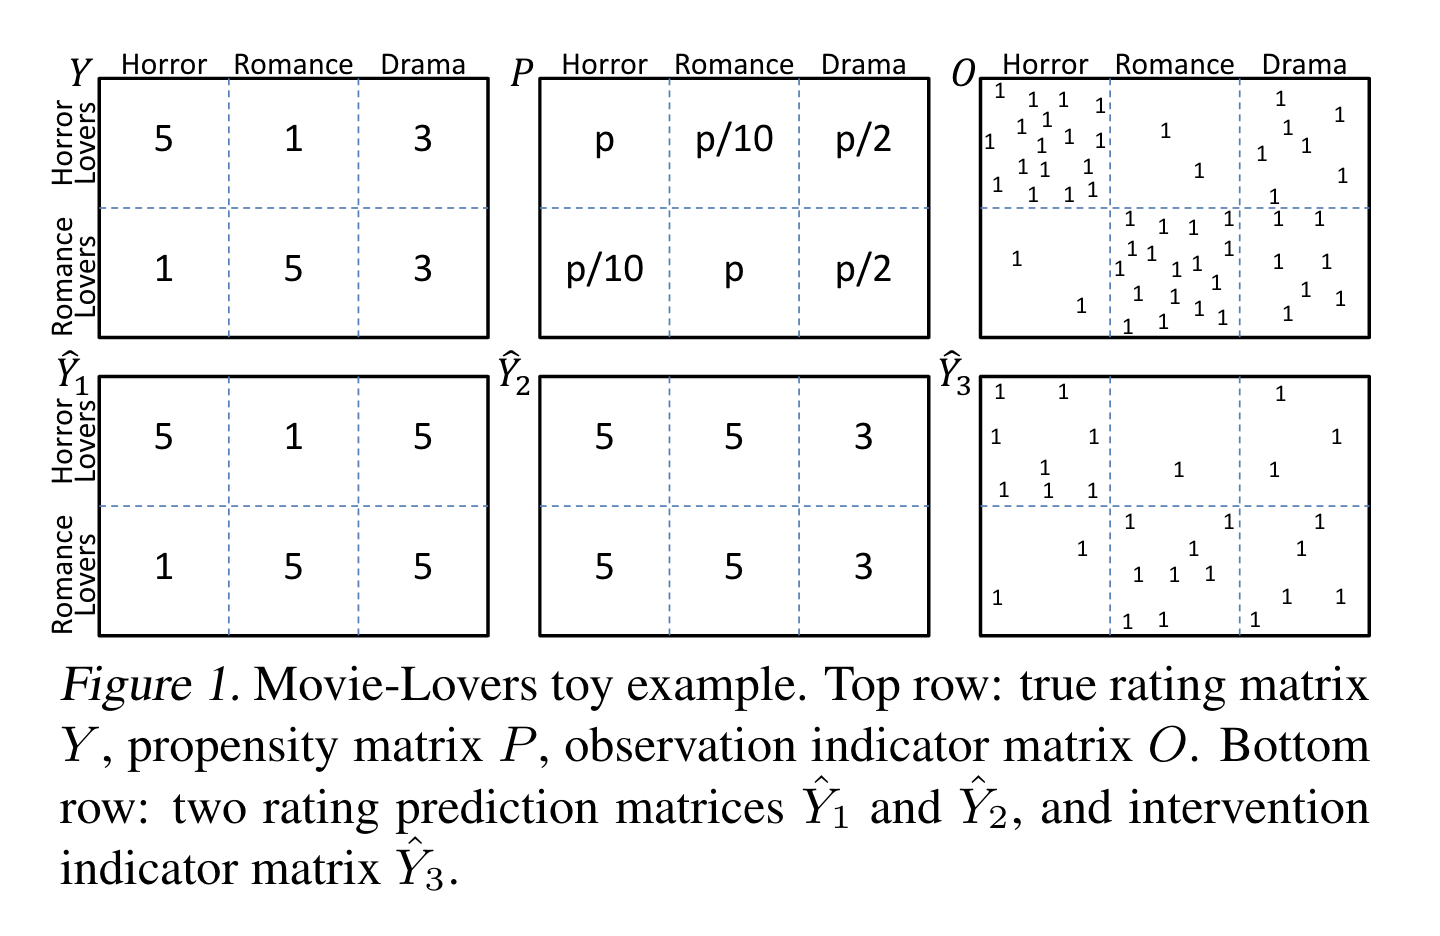
\includegraphics[scale=0.3]{images/bias-example.png}
\end{center}

\[
R(\hat Y) = \frac{1}{U I} \sum_u \sum_i \delta_{ui} (Y, \hat Y), \quad R_{naive}(\hat Y) = \frac{1}{N} \sum_{(u,i) \in D} \delta_{ui}(Y, \hat Y)
\]

\end{frame}

\begin{frame}{Смещения в рекомендациях \cite{BIAS}}

\begin{center}
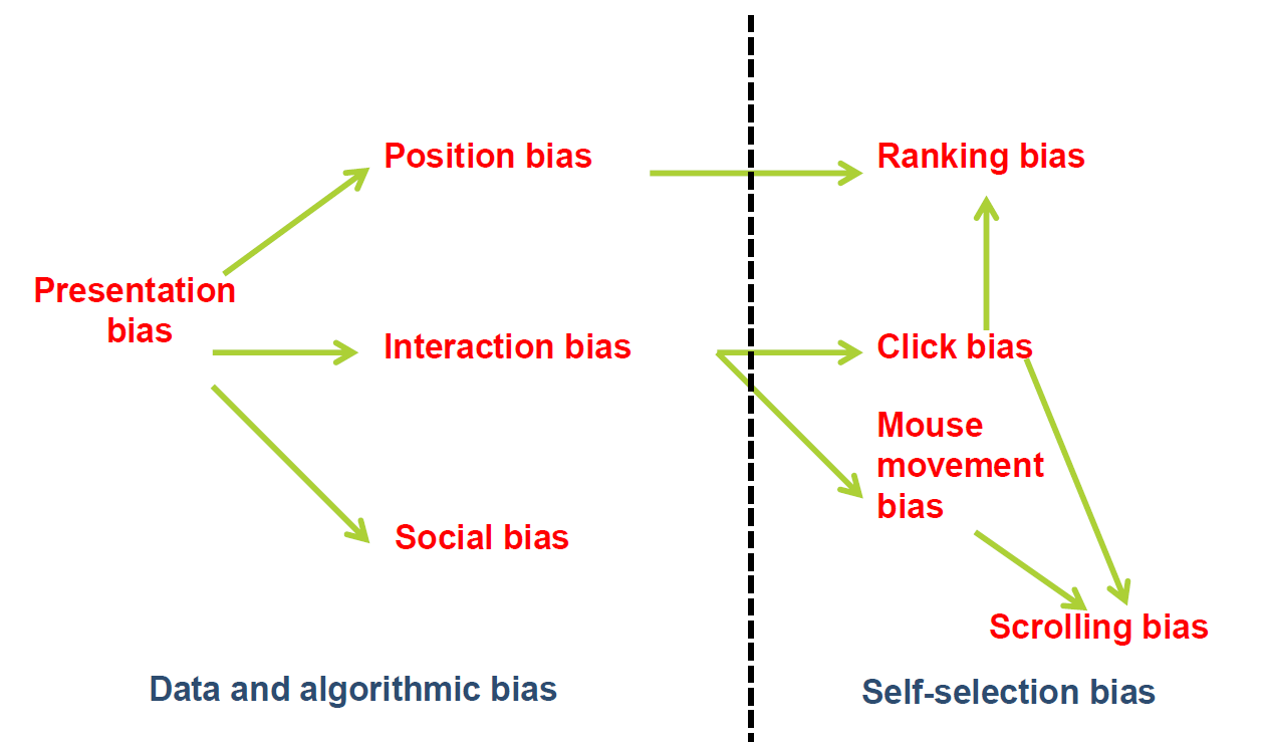
\includegraphics[scale=0.2]{images/bias.png}
\end{center}

\end{frame}

\begin{frame}{Inverse Propensity Scored Estimator \cite{TREATMENTS}}

$P_{ui} = P((u, i) \in D)$ -- вероятность, что пользователь $u$ поставит оценку айтему $i$

\[
R_{IPS}(\hat Y | P) = \frac{1}{U I} \sum_{(u,i) \in D} \frac{\delta_{ui}(Y, \hat Y)}{P_{ui}}
\]

\[
E_D [R_{IPS}(\hat Y | P)] = \frac{1}{U I} \sum_u \sum_i E_D\left[ \frac{\delta_{ui}(Y, \hat Y)}{P_{ui}} \mathbb{I}\{(u, i) \in D\}\right] = 
\]
\[
= \frac{1}{U I} \sum_u \sum_i \delta_{ui} (Y, \hat Y) = R(\hat Y) 
\]

\end{frame}

\begin{frame}{IPS Estimator: проблемы}

\begin{enumerate}
\item Когда $P_{ui}$ неизвестно, его приходится оценивать
\item Большая дисперсия при оценке $P_{ui}$
\item Непонятно, как быть с рекомендациями списков
\end{enumerate}

\end{frame}

\begin{frame}{Causal рекомендации}

\begin{tcolorbox}[colback=warn!5,colframe=warn!80,title=Традиционный рекомендер]
Посмотрит ли пользователь этот фильм, если известно что она смотрела в прошлом?
\end{tcolorbox}

\begin{tcolorbox}[colback=info!5,colframe=info!80,title=Causal рекомендер]
Посмотрит ли пользователь этот фильм, если мы его порекомендуем, и известно, что она смотрела в прошлом?
\end{tcolorbox}

\end{frame}

\begin{frame}{The Deconfounded Recommender \cite{DECONF}}

\vfill

\begin{tcolorbox}[colback=gray!5,colframe=gray!80,title=Confounder]
Переменная, которая влияет и на treatment assignment, и на outcome
\end{tcolorbox}

\begin{columns}
\begin{column}{0.4\textwidth}
\begin{center}
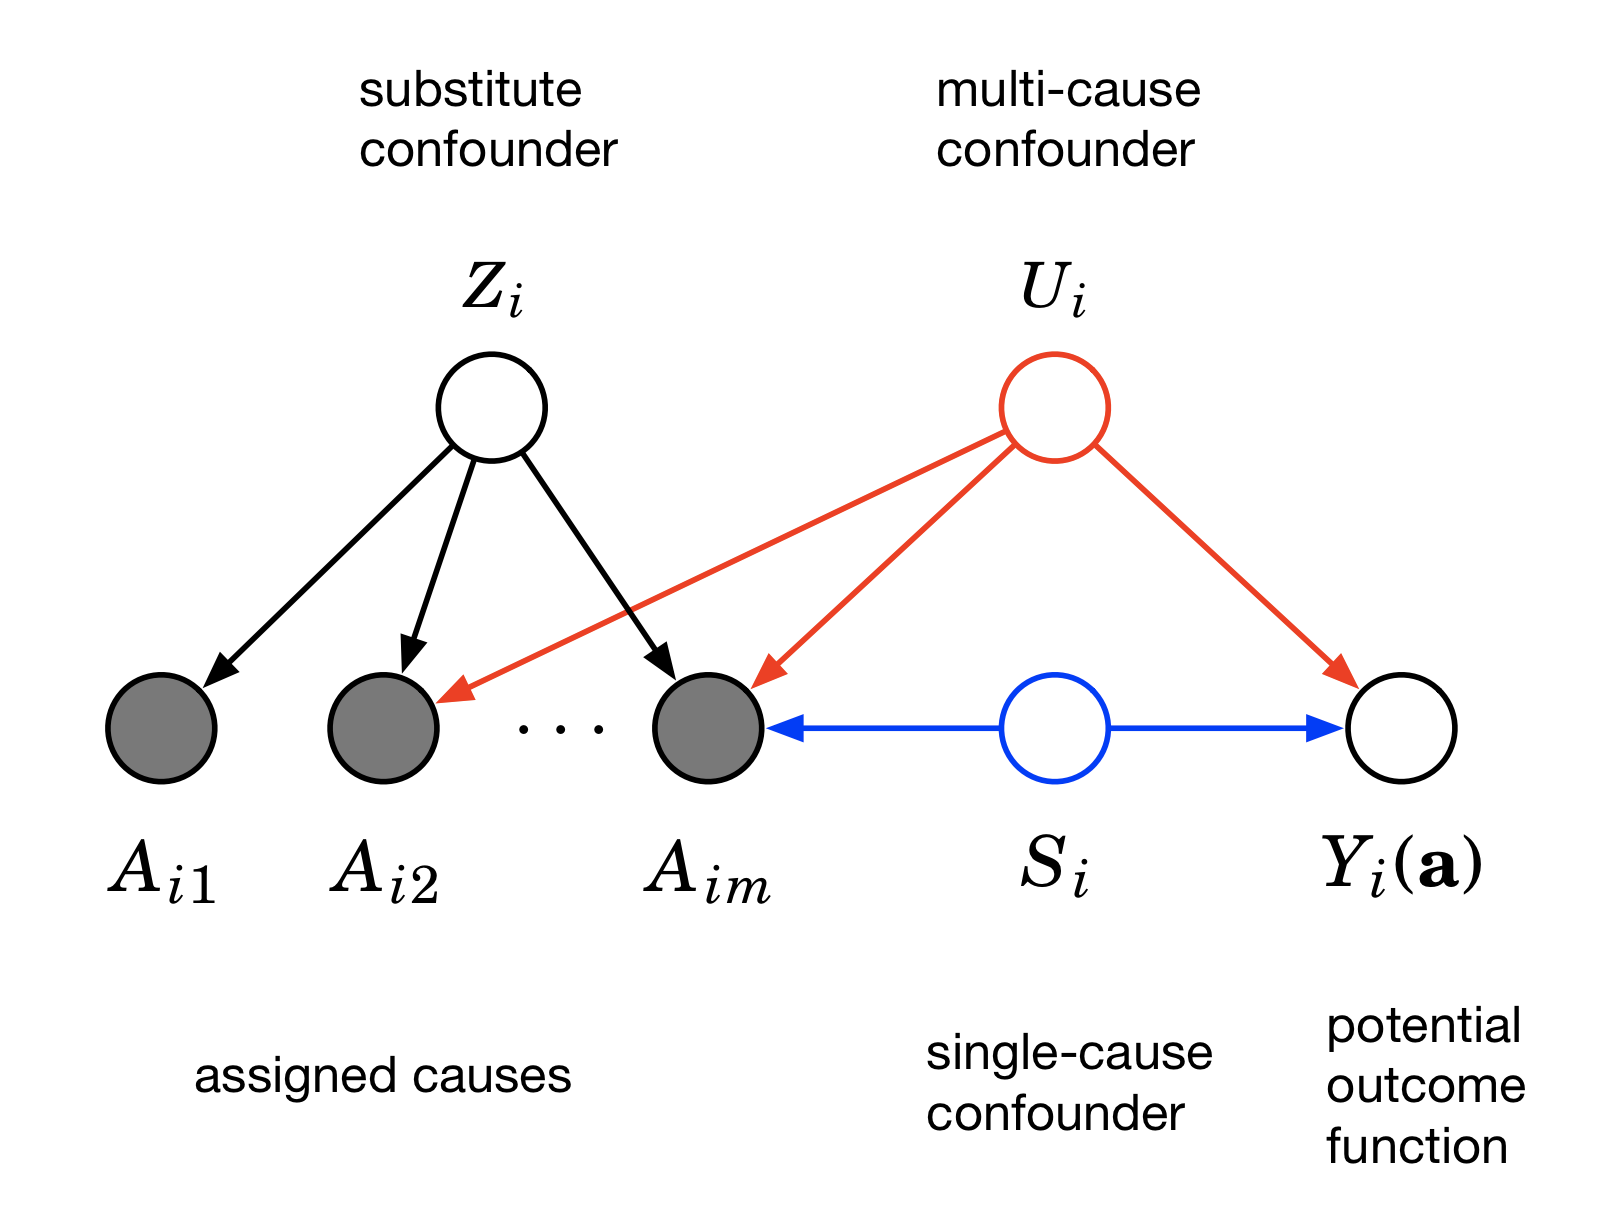
\includegraphics[scale=0.2]{images/blessings.png}
\end{center}
\end{column}

\begin{column}{0.5\textwidth}
\begin{enumerate}
\item Учим модель $p(z, a_1, \ldots, a_m)$
\item Оцениваем $E(z_j | a_{1j}, \ldots, a_{mj})$ для каждого наблюдения
\item Используем оценки для $z_j$ как признак в рекомендере
\end{enumerate}
\end{column}
\end{columns}

\end{frame}

\begin{frame}

\begin{center}
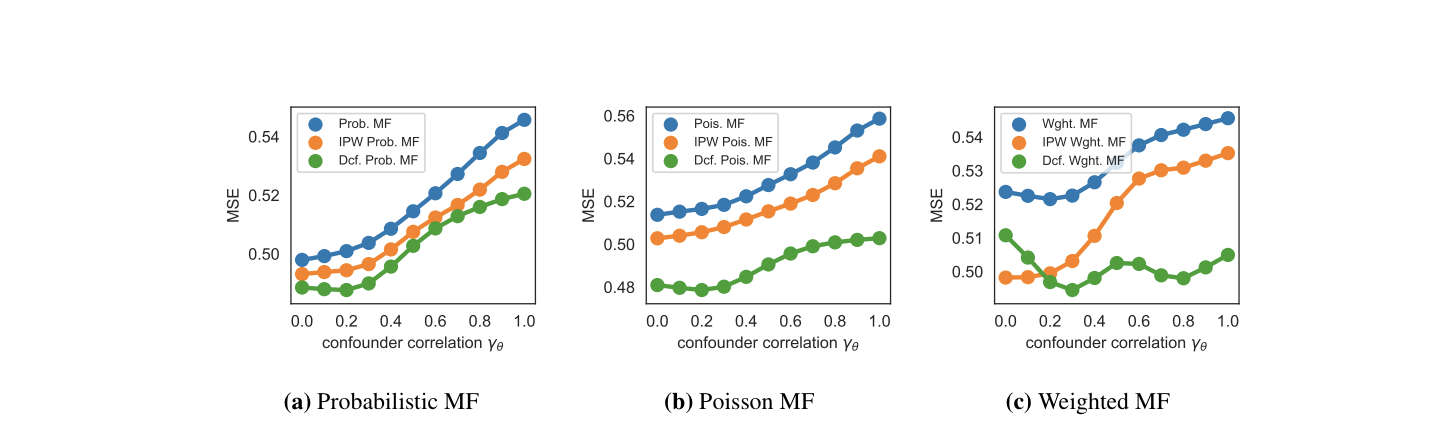
\includegraphics[scale=0.6]{images/deconf-result.png}
\end{center}

\end{frame}

\begin{frame}

\begin{tcolorbox}[colback=info!5,colframe=info!80,title=]
Из-за специфики сбора данных рекомендации подвержены смещениям. 
\end{tcolorbox}
\begin{tcolorbox}[colback=info!5,colframe=info!80,title=]
Существуют техники для корректировки, но они несовершенны.
\end{tcolorbox}

\end{frame}

\section{Итоги}

\begin{frame}{Итоги}

\begin{tcolorbox}[colback=info!5,colframe=info!80,title=]
При построении моделей мы делаем упрощающие предположения. Из-за этих предположений в продакшен системах могут возникать негативные эффекты. Эти эффекты нужно учитывать и пытаться исправить.
\end{tcolorbox}

\end{frame}

\begin{frame}
\begin{center}

\includegraphics[scale=0.55]{images/bye.jpeg}
\end{center}
\end{frame}

\begin{frame}[allowframebreaks]{Литература}

\bibliographystyle{amsalpha}
\bibliography{references.bib}

\end{frame}

\end{document}
